
\begin{itemize}
\item Ohm's Law works in AC exactly like it does in DC, just replace $R$ with $Z$: $\Delta V$ = $I Z$
\item Impedances of each component summarized in
  Table \ref{tab:impedanceSummary}
\item Equivalent impedance evaluated exactly as equivalent resistance:
  $Z_{series} = Z_1+Z_2$, $Z_{parallel}=\frac{Z_1\cdot Z_2}{Z_1+Z_2}$
\item Several shortcuts can be used for like elements:
  \begin{itemize}
  \item $C_{parallel}=C_1+C_2$, $C_{series} = \frac{C_1\cdot C_2}{C_1+C_2}$
  \item $L_{series} = L_1+L_2$, $L_{parallel} = \frac{L_1\cdot L_2}{L_1+L_2}$
  \end{itemize}
\end{itemize}
\ctable[
  cap = Impedance Element Summary,
  caption = A Summary of Elements Which Provide an Impedance,
  label = tab:impedanceSummary,
  pos = h
]{lVVV}{
  \tnote{Typical ceramic capacitors. Electrolytic capacitors have larger capacitance.}
  }{
  \FL
  & Capacitor                     & Inductor                & Resistor                     \\
  \midrule \vspace{-1em}\\ \vspace{-0.25em}
  Symbol
  & 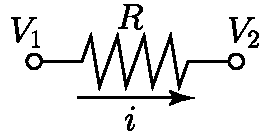
\includegraphics[height=30pt]{figures/ohmsLaw} 
  & 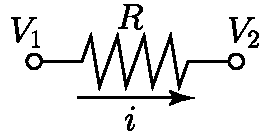
\includegraphics[height=30pt]{figures/ohmsLaw} 
  & 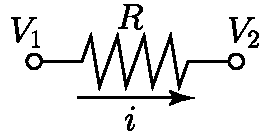
\includegraphics[height=30pt]{figures/ohmsLaw} \\
  Unit & Farad (F) & Henry (H) & Ohm ($\Omega$)      \\ \vspace{0.25 em}
  Typical Values
  & 0.1 pF -- 0.5 mF\tmark
  & 0.1 $\mu$H -- 10 mH
  & 10 $\Omega$ -- 1 G$\Omega$ \\ \vspace{0.5 em}
  Impedance
  & $\displaystyle Z_C=\frac{1}{j \omega C}$
  & $\displaystyle Z_L = j \omega L$
  & $\displaystyle Z_R = R$                    \\ 
  Energy Storage
  &  $\displaystyle E_C = \frac{1}{2} CV^2$
  & $\displaystyle E_L = \frac{1}{2}Li^2$
  & N/A 
\LL
}



%% Examples
\begin{itemize}
\item Simple RL circuit (series)
  \begin{itemize}
  \item $V = 10 \cos (500 t + \pi / 4)$ V
  \item $R = 100 \Omega$
  \item $L = 50 mH$
  \item Find I
  \end{itemize}
\item Simple RLC circuit (RL parallel, C series)
  \begin{itemize}
  \item $I = 40 \cos (2400 t)$ mA
  \item $R = 1000 \Omega$
  \item $L = 100 mH$
  \item $C = 15 \mu F$
  \item Find V
  \end{itemize}
\end{itemize}
